\subsection{Red de grafos generada por el RNA}
	
 	La información exportada en el Código \ref{lst:EJ1_4} (Infrastructure.RNA), Código \ref{lst:EJ1_5} (SafePoint.RNA), Código \ref{lst:EJ1_6} (Signalling.RNA) y Código \ref{lst:EJ1_7} (Routes.RNA) es resumida de forma gráfica por el RNA para una mejor interpretación. El RNA combina la información de la clase \textit{netRelations} (contenida en Infrastructure.RNA y SafePoint.RNA), la clase \textit{signalsIS} (contenida en Signalling.RNA) y la clase \textit{Routes} (contenida en Routes.RNA) mediante el uso de las bibliotecas networkx \cite{NETWORKX} y graphviz \cite{GRAPHVIZ}. La biblioteca networkx es utilizada por el RNA para crear, procesar y analizar la red de grafos definida en base a los datos de la clase \textit{netRelations}, siguiendo los pasos explicados en la Sección \ref{sec:grafos}. Aunque la biblioteca networkx permite graficar los resultados, se limitan a representar las relaciones nodo/arista, mientras que railML contiene datos muchos más detallados. La biblioteca graphviz es una herramienta mucho mas potente a la hora de representar gráficamente un grafo y es posible una mayor personalización de las figuras obtenidas. Por ejemplo, la biblioteca graphviz permite incluir información relacionada a la infraestructura contenida en cada \textit{netElement}, lo cual enriquece la representación gráfica del análisis que realiza el RNA. El resultado de este resumen se ilustra en el diagrama de la Figura \ref{fig:EJ1_8}.

	\begin{figure}[H]
		\centering
		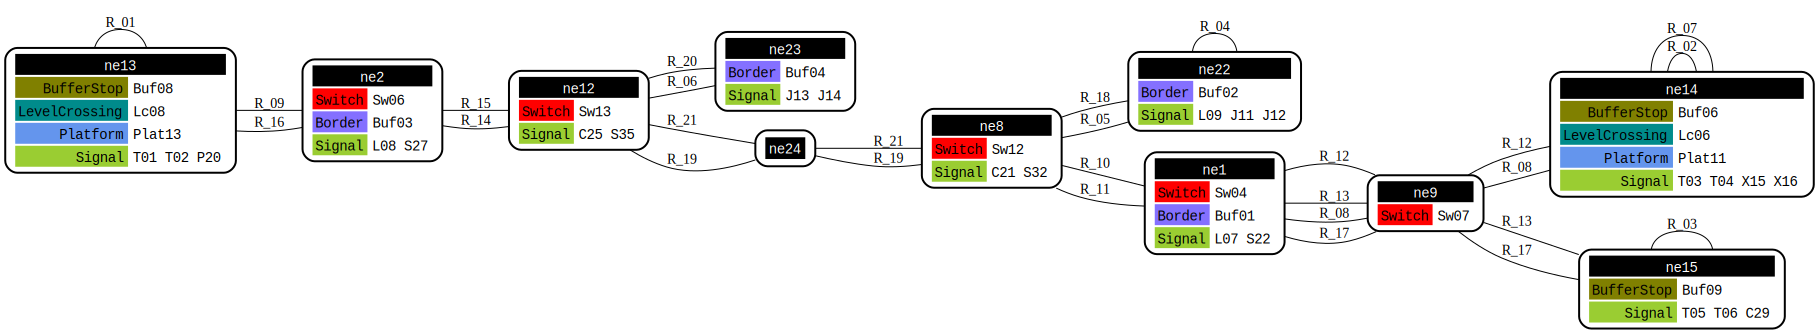
\includegraphics[origin = c, width=\textwidth]{Figuras/Graph_1}
		\centering\caption{Red de grafos generada por el RNA para el ejemplo 1.}
		\label{fig:EJ1_8}
	\end{figure}
	
	Cada nodo del grafo de la Figura \ref{fig:EJ1_8} corresponde a un \textit{netElement} de la Figura \ref{fig:EJ1_1}. En cada nodo se listan todos los elementos ferroviarios contenidos por el \textit{netElement}. Las aristas del grafo son las rutas que los conectan. De esta manera, es posible detectar visualmente cualquier nodo aislado de la red o nodos que solo son accedidos en un sentido. Por ejemplo, si entre dos nodos no existe una cantidad par de rutas, entonces solamente se puede circular entre esos nodos en un solo sentido.